\chapter{Acceptance test} \label{chap:acceptanceTest}

The system is tested to see if it fulfills the requirements put up (\chapref{chap:requirements}).

Nadir pointing capability is tested by turning on the linear attitude controller of a satellite with initial attitude and angular velocity deviating from the reference. After reducing the initial error, the tracking error stays below $1^o$, as shown in figure \ref{fig:angle_error.}.

\begin{figure}[H]
	\centering
	%	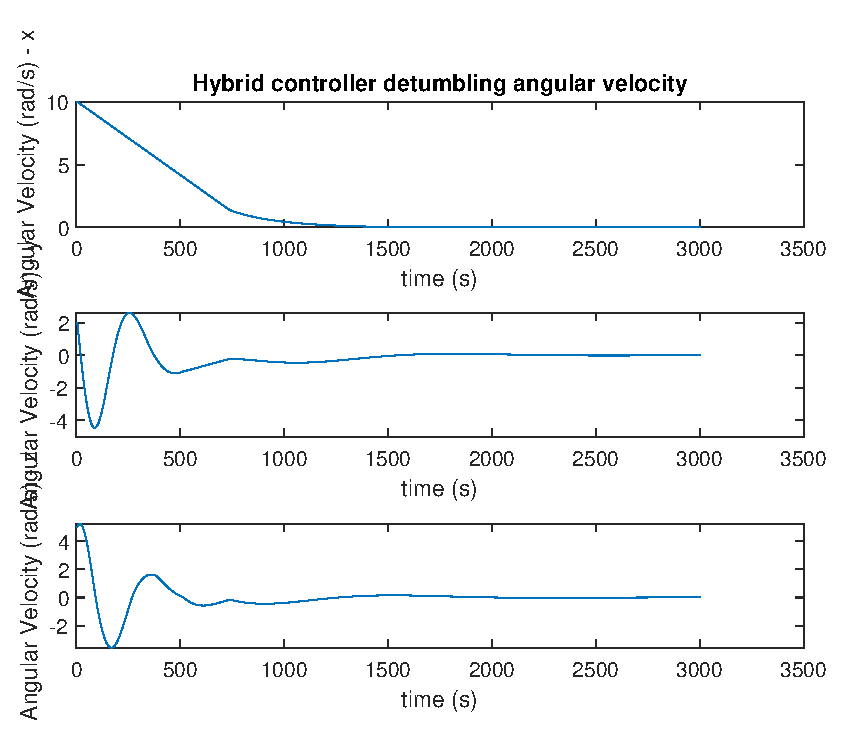
\includegraphics[width=0.7\linewidth]{figures/detumbling3}
	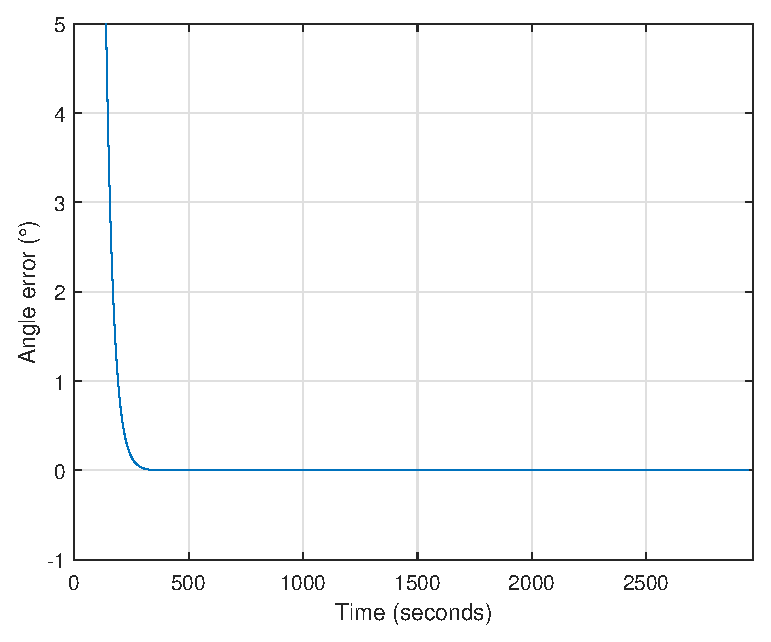
\includegraphics[width=0.7\linewidth]{figures/angle_error}
	\caption{Tracking error during nadir pointing}
	\label{fig:angle_error}
\end{figure}

Earth station tracking is  tested in a scenario where the satellite flies right over the station. This is the closest the satellite in orbit can get to the Earth station, leading to maximum torque demand. The tracking error is kept below  $1^o$, with error peaks appearing during flyover. Figures \ref{fig:angle_error2} and \ref{fig:torque_stationTrack} present the tracking error and torque demand arising during station tracking.

\begin{figure}[H]
	\centering
	%	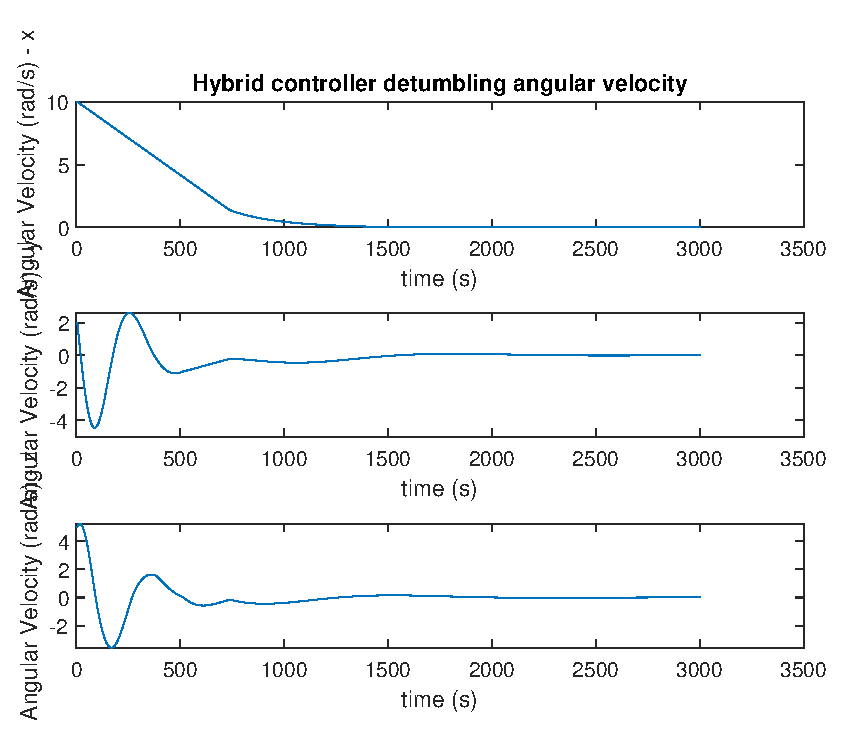
\includegraphics[width=0.7\linewidth]{figures/detumbling3}
	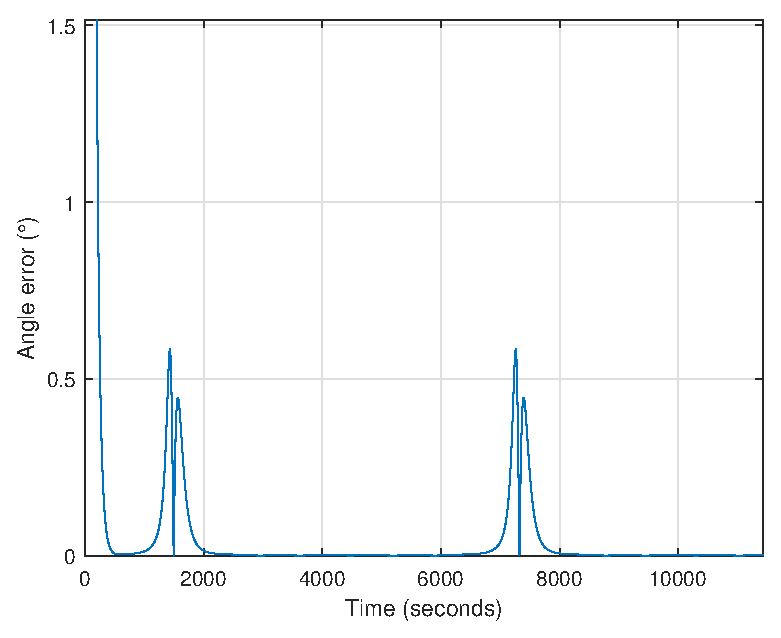
\includegraphics[width=0.7\linewidth]{figures/angle_error_stationTrack}
	\caption{Tracking error during Earth station pointing. The satellite flies over the station.}
	\label{fig:angle_error2}
\end{figure}


\begin{figure}[H]
	\centering
	%	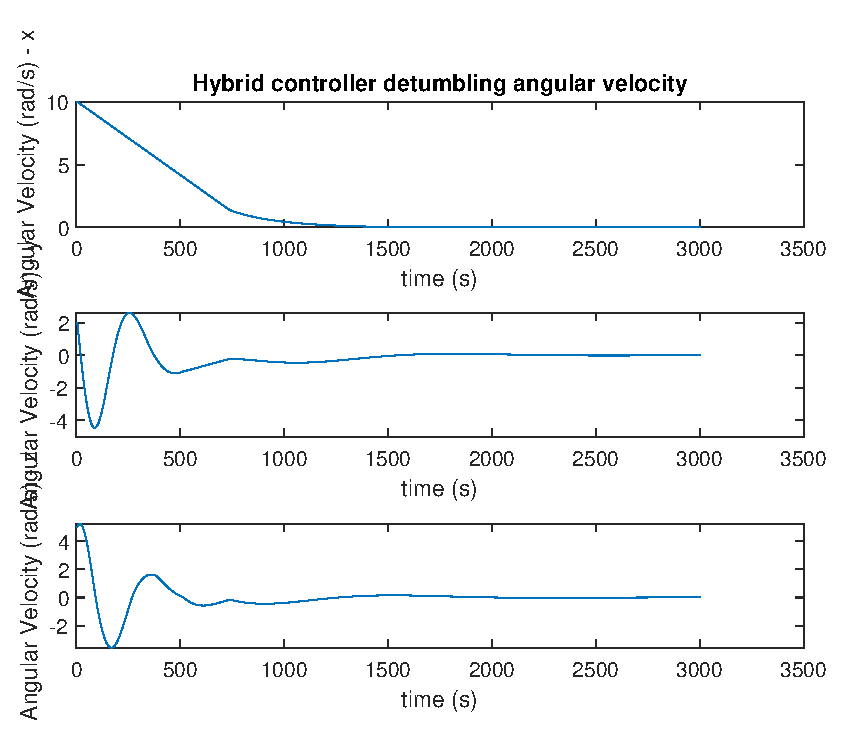
\includegraphics[width=0.7\linewidth]{figures/detumbling3}
	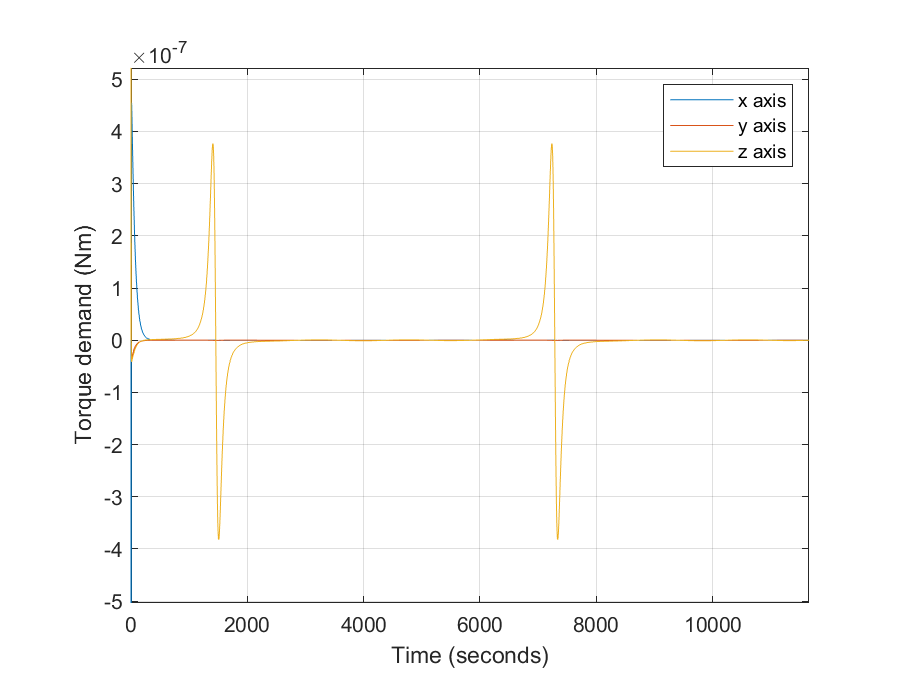
\includegraphics[width=0.7\linewidth]{figures/torque_stationTrack}
	\caption{Torque demand $\vec{u}$ during Earth station pointing. The satellite flies over the station.}
	\label{fig:torque_stationTrack}
\end{figure}

\begin{figure}[H]
	\centering
	%	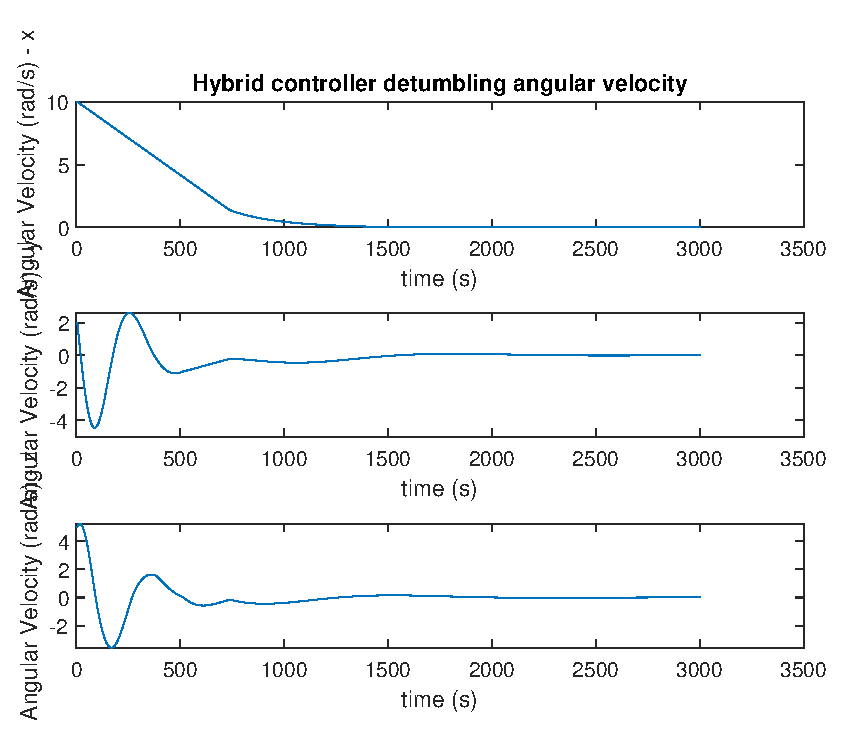
\includegraphics[width=0.7\linewidth]{figures/detumbling3}
	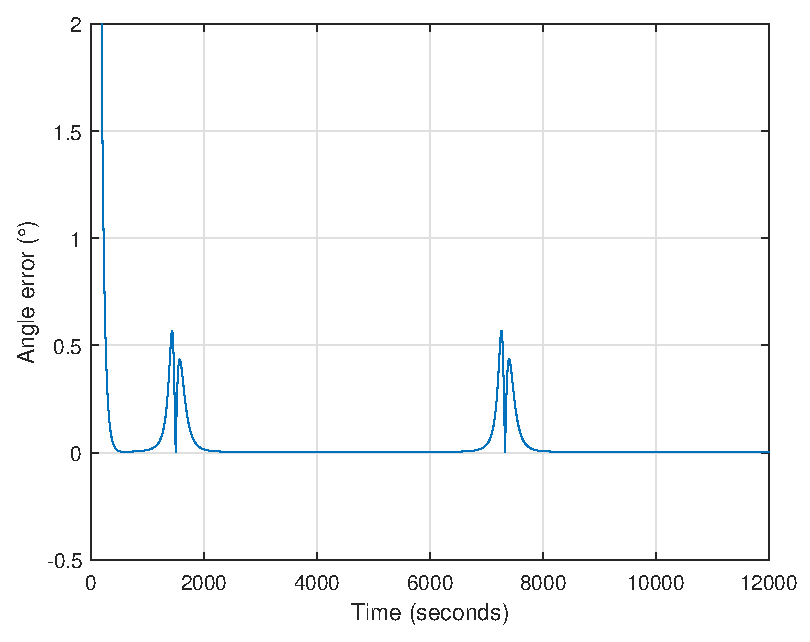
\includegraphics[width=0.7\linewidth]{figures/faultyangerror}
	\caption{Tracking error during Earth station pointing using the linear controller. The satellite flies over the station. The 3rd reaction wheel is faulty and switched off.}
	\label{fig:angle_error2}
\end{figure}


%\subsection{1. The formation shall be able to maintain a given angle within 45$^{\circ}$.}
%The
